% ==============================================================
%  END-SEMESTER PRESENTATION (3 slides, matches midsem PPT layout)
%  Project : Fast Authentication Between UAVs (PUF-based)
%  Author  : Md Ziyad Hussain (Roll No. 2301128)
%  Course  : CS300  |  Supervisor: Dr. Rakesh Matam
% ==============================================================
\documentclass[aspectratio=169,10pt]{beamer}

\usepackage[T1]{fontenc}
\usepackage{lmodern}
\renewcommand{\familydefault}{\sfdefault}
\usepackage{tikz}
\usetikzlibrary{positioning}
\usepackage{pgfplots}
\pgfplotsset{compat=1.18}
\usepackage{xcolor}
\usepackage{colortbl}
\usepackage{enumitem}
\usepackage[hidelinks]{hyperref}

% ---------- Colours sampled from the midsem PPT ----------
\definecolor{HeaderBlue}{HTML}{5B9BD5}     % main accent (top band) -- sky blue
\definecolor{FooterDark}{HTML}{8FAADC}     % darker -- left footer cell
\definecolor{FooterMid}{HTML}{B4C7E7}      % medium -- middle footer cell
\definecolor{FooterBlue}{HTML}{D9E2F3}     % lightest -- right footer cell
\definecolor{SubHeadBlue}{HTML}{D9E2F3}
\definecolor{LogoNavy}{HTML}{063872}
\definecolor{BodyBlack}{HTML}{000000}

% ---------- Strip beamer chrome ----------
\setbeamertemplate{navigation symbols}{}
\setbeamertemplate{footline}{}
\setbeamertemplate{headline}{}
\setbeamercolor{normal text}{fg=BodyBlack}
\setbeamerfont{itemize/enumerate body}{size=\scriptsize}
\setbeamerfont{itemize/enumerate subbody}{size=\tiny}

% ---------- Geometry constants -------
% ---------- Geometry constants -------------
\newcommand{\HeaderHeight}{1.55cm}
\newcommand{\FooterHeight}{0.62cm}

% ---------- Header band ----------
% \slidehead{<title>}{<fill colour>}{<text colour>}
\newcommand{\slidehead}[3]{%
  \begin{tikzpicture}[remember picture,overlay]
    \fill[#2] ([yshift=0pt]current page.north west)
              rectangle ([yshift=-\HeaderHeight]current page.north east);
    \node[anchor=west,text=#3,font=\LARGE\bfseries,inner sep=0pt]
      at ([xshift=0.55cm,yshift=-\HeaderHeight/2]current page.north west) {#1};
    % logo flush to top-right corner (no inset)
    \node[anchor=north east,inner sep=0pt]
      at (current page.north east)
      {
\includegraphics[height=\HeaderHeight]{image.png}};
  \end{tikzpicture}%
}

% ---------- Footer band (3 shaded cells) ----------
% \slidefoot{<right column text>}
\newcommand{\slidefoot}[1]{%
  \begin{tikzpicture}[remember picture,overlay]
    % three shaded cells (darker -> lighter, left -> right)
    \fill[FooterDark] ([xshift=0cm,    yshift=0pt]current page.south west)
                      rectangle ([xshift=4.6cm,  yshift=\FooterHeight]current page.south west);
    \fill[FooterMid]  ([xshift=4.6cm,  yshift=0pt]current page.south west)
                      rectangle ([xshift=8.6cm,  yshift=\FooterHeight]current page.south west);
    \fill[FooterBlue] ([xshift=8.6cm,  yshift=0pt]current page.south west)
                      rectangle ([xshift=0pt,    yshift=\FooterHeight]current page.south east);
    \node[anchor=west,font=\footnotesize\bfseries,text=BodyBlack]
      at ([xshift=0.25cm,yshift=\FooterHeight/2]current page.south west)
      {Name: Md Ziyad Hussain};
    \node[anchor=west,font=\footnotesize\bfseries,text=BodyBlack]
      at ([xshift=4.85cm,yshift=\FooterHeight/2]current page.south west)
      {Roll No: 2301128};
    \node[anchor=west,font=\footnotesize\bfseries,text=BodyBlack]
      at ([xshift=8.85cm,yshift=\FooterHeight/2]current page.south west)
      {#1};
  \end{tikzpicture}%
}

% Tight itemize spacing with square bullets like the PPT
\setlist[itemize,1]{leftmargin=1.4em, itemsep=2pt, topsep=2pt, parsep=0pt,
                    label=\textcolor{BodyBlack}{\rule[0.35ex]{0.55ex}{0.55ex}}}
\setlist[itemize,2]{leftmargin=1.4em, itemsep=2pt, topsep=2pt, parsep=0pt,
                    label=\textcolor{BodyBlack}{\rule[0.35ex]{0.45ex}{0.45ex}}}

% ==============================================================
\begin{document}

% ---------------- SLIDE 1 ----------------
\begin{frame}[t]
  \slidehead{Fast Authentication Between UAVs}{HeaderBlue}{white}
  \slidefoot{Supervisor: Dr.\ Rakesh Matam}

  \vspace{1.20cm}
  {\large\bfseries Introduction:}
  \begin{itemize}
    \item UAVs are widely used in surveillance, delivery and defence -- all need secure communication.
    \item Authentication between UAVs and the Ground Station prevents impersonation, replay and cloning attacks.
    \item Physical Unclonable Functions (PUFs) give hardware-based identity \textbf{without storing any key} -- ideal for resource-constrained UAVs.
  \end{itemize}

  \vspace{0.20cm}
  {\large\bfseries Motivation:}
  \begin{itemize}
    \item RSA/ECC need 5--10$\times$ more computation \& energy -- unsuitable for battery-powered UAVs.
    \item Stored secret keys are vulnerable when a UAV is physically captured.
    \item Need a \textbf{fast peer-to-peer} authentication mechanism for UAV swarms, independent of the Ground Station.
  \end{itemize}
\end{frame}

% ---------------- SLIDE 2 ----------------
\begin{frame}[t]
  \slidehead{Existing work / Literature review:}{SubHeadBlue}{BodyBlack}
  \slidefoot{Project Title: Fast Authentication Between UAVs}

  \vspace{1.20cm}
  \begin{columns}[T]
    \begin{column}{0.55\linewidth}
      \footnotesize
      \begin{itemize}[itemsep=2pt,topsep=2pt,parsep=0pt]
        \item PKI / symmetric protocols give strong security but \textbf{high compute overhead} -- impractical for small UAVs.
        \item Lightweight schemes use hash-and-XOR (SPONGENT, SHA-3) to cut compute by \textbf{50--90\%}.
        \item PUF-based methods derive identity from \textbf{manufacturing variations} -- no key stored on the UAV.
      \end{itemize}

      \vspace{0.15cm}
      {\normalsize\bfseries Gaps in existing work:}
      \begin{itemize}[itemsep=2pt,topsep=2pt,parsep=0pt]
        \item RSA / ECC need too much CPU for small UAVs.
        \item Stored-key protocols leak secrets when UAV is captured.
        \item Few schemes give \textbf{fast peer-to-peer} UAV auth without GS.
      \end{itemize}
    \end{column}
    \begin{column}{0.43\linewidth}
      \centering
      {\scriptsize\bfseries\color{LogoNavy}Compute time on Cortex-M4 @ 168 MHz (per auth)}\\[2pt]
      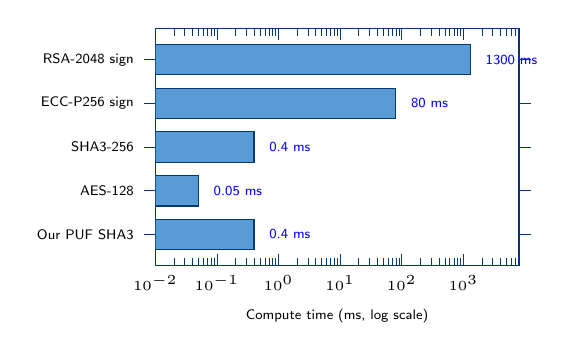
\begin{tikzpicture}
        \begin{axis}[
          width=6.2cm, height=4.6cm,
          xbar, bar width=11pt,
          xmode=log, log origin=infty,
          xmin=0.01, xmax=8000,
          xlabel={Compute time (ms, log scale)},
          symbolic y coords={Our PUF SHA3,AES-128,SHA3-256,ECC-P256 sign,RSA-2048 sign},
          ytick=data,
          y tick label style={font=\tiny},
          x tick label style={font=\tiny},
          xlabel style={font=\tiny},
          point meta=explicit symbolic,
          nodes near coords,
          nodes near coords style={font=\tiny,anchor=west,xshift=2pt},
          enlarge y limits=0.18,
          axis line style={LogoNavy},
          tick style={LogoNavy},
        ]
        \addplot+[fill=HeaderBlue,draw=LogoNavy] coordinates {
          (1300,RSA-2048 sign)        [1300 ms]
          (80,ECC-P256 sign)          [80 ms]
          (0.4,SHA3-256)              [0.4 ms]
          (0.05,AES-128)              [0.05 ms]
          (0.4,Our PUF SHA3)          [0.4 ms]
        };
        \end{axis}
      \end{tikzpicture}\\[1pt]
      {\tiny RSA/ECC: \href{https://www.wolfssl.com/docs/benchmarks/}{\textit{wolfSSL Cortex-M4 benchmarks}}. SHA3/AES: \href{https://keccak.team/sw_performance.html}{\textit{Keccak Team SUPERCOP}} \& \href{https://tls.mbed.org/benchmarks}{\textit{mbedTLS}} reports.}
    \end{column}
  \end{columns}
\end{frame}

% ---------------- SLIDE 3 ----------------
\begin{frame}[t]
  \slidehead{Work Done till date:}{SubHeadBlue}{BodyBlack}
  \slidefoot{Project Title: Fast Authentication Between UAVs}

  \vspace{1.05cm}
  \begin{columns}[T]
    \begin{column}{0.54\linewidth}
      {\scriptsize\bfseries\color{LogoNavy}My work:}\vspace{-1pt}
      {\tiny\begin{itemize}[itemsep=0pt,topsep=0pt,parsep=0pt,leftmargin=1.0em,label=\textcolor{BodyBlack}{\rule[0.3ex]{0.45ex}{0.45ex}}]
        \item Implemented \textbf{4-phase PUF auth} in \textbf{OMNeT++ 6.3} (10 UAVs + 1 GS); \textbf{Arbiter PUF + BCH(255,131,18)} fuzzy extractor; SHA3-256 / SPONGENT-160 modes.
        \item End-to-end benchmark: compute, network, energy, area; predicted Pi-4 / Cortex-M4 / ASIC numbers.
      \end{itemize}}\vspace{-3pt}

      {\tiny\bfseries\color{LogoNavy}SHA3-256 vs SPONGENT-160 -- detailed comparison:}\\[1pt]
      {\tiny
      \renewcommand{\arraystretch}{0.95}
      \setlength{\tabcolsep}{2pt}
      \begin{tabular}{|l|c|c|}
        \hline
        \rowcolor{SubHeadBlue}
        \textbf{Metric} & \textbf{SHA3-256} & \textbf{SPONGENT-160} \\
        \hline
        Gate area (130 nm)\,$^{[1,2]}$         & $\sim$15{,}000 GE    & \textbf{1{,}329 GE} \\
        \hline
        Energy / hash (HW)\,$^{[1,2]}$         & $\sim$2.0 nJ         & \textbf{$\sim$0.66 nJ} \\
        \hline
        Power (HW @100 kHz)\,$^{[1]}$          & $\sim$30 \textmu W   & \textbf{$\sim$1.6 \textmu W} \\
        \hline
        Throughput (HW @100 kHz)               & 8 kbps               & 0.81 kbps \\
        \hline
        \rowcolor{FooterBlue}
        Compute -- Laptop x86-64 (\emph{ours}) & \textbf{0.009 ms}    & 14.07 ms \\
        \hline
        \rowcolor{FooterBlue}
        Compute -- RaspPi 4 (A72)\,$^{[3]}$    & \textbf{$\sim$0.05 ms} & $\sim$80 ms \\
        \hline
        \rowcolor{FooterBlue}
        Compute -- Cortex-M4\,$^{[3]}$         & $\sim$0.4 ms         & $\sim$200 ms \\
        \hline
        ASIC HW estimate\,$^{[1,2]}$           & $\sim$0.01 ms        & \textbf{$\sim$0.05 ms} \\
        \hline
        \rowcolor{FooterMid}
        Network delay (\emph{ours, OMNeT++})   & 0.665 / 0.467 ms     & 0.665 / 0.467 ms \\
        \hline
      \end{tabular}}\\[2pt]
      {\tiny [1] \href{https://doi.org/10.1007/978-3-642-23951-9_21}{Bogdanov et al., \textit{SPONGENT}, CHES'11}. \,[2] \href{https://doi.org/10.6028/NIST.FIPS.202}{FIPS-202}. \,[3] \href{https://www.wolfssl.com/docs/benchmarks/}{wolfSSL bench}.}\vspace{1pt}

      {\scriptsize\bfseries\color{LogoNavy}Key summary:}\vspace{-1pt}
      {\tiny\begin{itemize}[itemsep=0pt,topsep=0pt,parsep=0pt,leftmargin=1.0em,label=\textcolor{BodyBlack}{\rule[0.3ex]{0.45ex}{0.45ex}}]
        \item \textbf{SHA3-256} fastest in software; \textbf{SPONGENT-160} 11$\times$ smaller silicon \& 3$\times$ less energy/hash (built for ASIC).
        \item Both use \textbf{$\sim$1000$\times$ less energy than RSA-2048}, $\sim$80$\times$ less than ECC-P256.
        \item \textbf{Total auth = compute + network} (OMNeT++ stadium, 10 UAVs):
        \begin{itemize}[itemsep=0pt,topsep=0pt,parsep=0pt,leftmargin=1.0em,label=\textcolor{BodyBlack}{\textendash}]
          \item P2 (UAV$\leftrightarrow$GS): SHA3 \textbf{0.007+0.665=0.67 ms}; SPONGENT \textbf{6.70+0.665=7.37 ms}.
          \item P3 (UAV$\leftrightarrow$UAV): SHA3 \textbf{0.009+0.467=0.48 ms}; SPONGENT \textbf{14.07+0.467=14.54 ms}.
        \end{itemize}
        \item \textbf{100\% success}, 430 B payload, no key storage; \emph{no MAC-layer contention modelled} (lower bound).
      \end{itemize}}
    \end{column}
    \begin{column}{0.44\linewidth}
      \centering
      {\tiny\bfseries\color{LogoNavy}Compute time per hash across devices (ms, log)}\\[-1pt]
      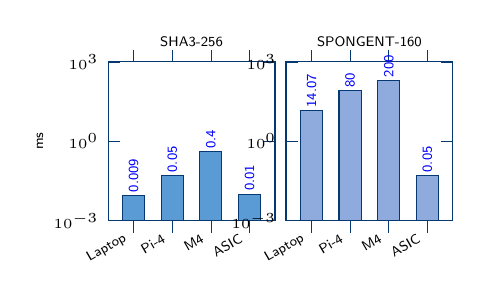
\begin{tikzpicture}
        \begin{axis}[
          name=ax1,
          width=3.7cm, height=3.6cm,
          ybar, bar width=8pt,
          ymode=log, log origin=infty,
          ymin=0.001, ymax=1000,
          ylabel={ms}, ylabel style={font=\tiny,yshift=-3pt},
          title={\tiny SHA3-256}, title style={yshift=-4pt},
          symbolic x coords={Laptop,Pi-4,M4,ASIC},
          xtick=data,
          x tick label style={font=\tiny,rotate=30,anchor=east},
          y tick label style={font=\tiny},
          enlarge x limits=0.22,
          point meta=explicit symbolic,
          nodes near coords, nodes near coords style={font=\tiny,rotate=90,anchor=west,inner sep=1pt},
          axis line style={LogoNavy}, tick style={LogoNavy},
        ]
        \addplot+[fill=HeaderBlue,draw=LogoNavy] coordinates {
          (Laptop,0.009)[0.009] (Pi-4,0.05)[0.05] (M4,0.4)[0.4] (ASIC,0.01)[0.01]
        };
        \end{axis}
        \begin{axis}[
          at={(ax1.east)}, anchor=west, xshift=4pt,
          width=3.7cm, height=3.6cm,
          ybar, bar width=8pt,
          ymode=log, log origin=infty,
          ymin=0.001, ymax=1000,
          title={\tiny SPONGENT-160}, title style={yshift=-4pt},
          symbolic x coords={Laptop,Pi-4,M4,ASIC},
          xtick=data,
          x tick label style={font=\tiny,rotate=30,anchor=east},
          y tick label style={font=\tiny},
          enlarge x limits=0.22,
          point meta=explicit symbolic,
          nodes near coords, nodes near coords style={font=\tiny,rotate=90,anchor=west,inner sep=1pt},
          axis line style={LogoNavy}, tick style={LogoNavy},
        ]
        \addplot+[fill=FooterDark,draw=LogoNavy] coordinates {
          (Laptop,14.07)[14.07] (Pi-4,80)[80] (M4,200)[200] (ASIC,0.05)[0.05]
        };
        \end{axis}
      \end{tikzpicture}\\[-2pt]
      {\tiny\itshape Values in ms. SPONGENT wins \emph{only} in silicon (\href{https://doi.org/10.1007/978-3-642-23951-9_21}{Bogdanov, CHES'11}).}

      \vspace{0.02cm}
      {\tiny\bfseries\color{LogoNavy}Energy per auth on UAV (nJ, log) -- vs other crypto}\\[-1pt]
      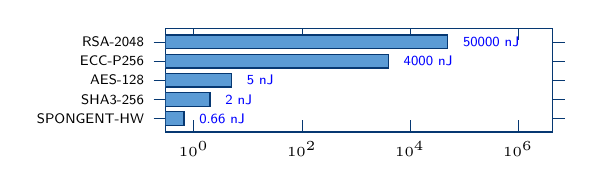
\begin{tikzpicture}
        \begin{axis}[
          width=6.5cm, height=2.9cm,
          xbar, bar width=5pt,
          xmode=log, log origin=infty,
          xmin=0.3, xmax=2000000,
          enlarge x limits={upper,value=0.05},
          symbolic y coords={SPONGENT-HW,SHA3-256,AES-128,ECC-P256,RSA-2048},
          ytick=data,
          y tick label style={font=\tiny},
          x tick label style={font=\tiny},
          point meta=explicit symbolic,
          nodes near coords, nodes near coords style={font=\tiny,anchor=west,xshift=2pt},
          enlarge y limits=0.18,
          axis line style={LogoNavy}, tick style={LogoNavy},
        ]
        \addplot+[fill=HeaderBlue,draw=LogoNavy] coordinates {
          (50000,RSA-2048)  [50000 nJ]
          (4000,ECC-P256)   [4000 nJ]
          (5,AES-128)       [5 nJ]
          (2,SHA3-256)      [2 nJ]
          (0.66,SPONGENT-HW)[0.66 nJ]
        };
        \end{axis}
      \end{tikzpicture}\\[-2pt]
      {\tiny\itshape RSA/ECC/AES: \href{https://www.wolfssl.com/docs/benchmarks/}{wolfSSL Cortex-M bench}.}
    \end{column}
  \end{columns}
\end{frame}

\end{document}
